\chapter{Конструкторский раздел}

\section{Проектирование базы данных}
\subsection{Таблицы базы данных}
В соответствии с ER-диаграммой системы, изображенной на рисунке \ref{img:er-dia}, база данных приложения хранит следующие таблицы:
\begin{enumerate}
	\item Таблица пользователей --- UserDB;
	\item Таблица промокодов --- PromoDB;
	\item Таблица товаров --- ProductDB;
	\item Таблица заказов --- OrderDb;
	\item Таблица деталей заказов --- ItemOrderDB;
	\item Таблица корзины --- CartDB;
	\item Таблица деталей корзины --- ItemCartDB;
	\item Таблица связи многие к многим --- UserPromoDB;
\end{enumerate}
\newpage
На рисунке \ref{img:er-db} представлена диаграмма разрабатываемой базы данных.
\begin{figure}[ht!]
	\centering
	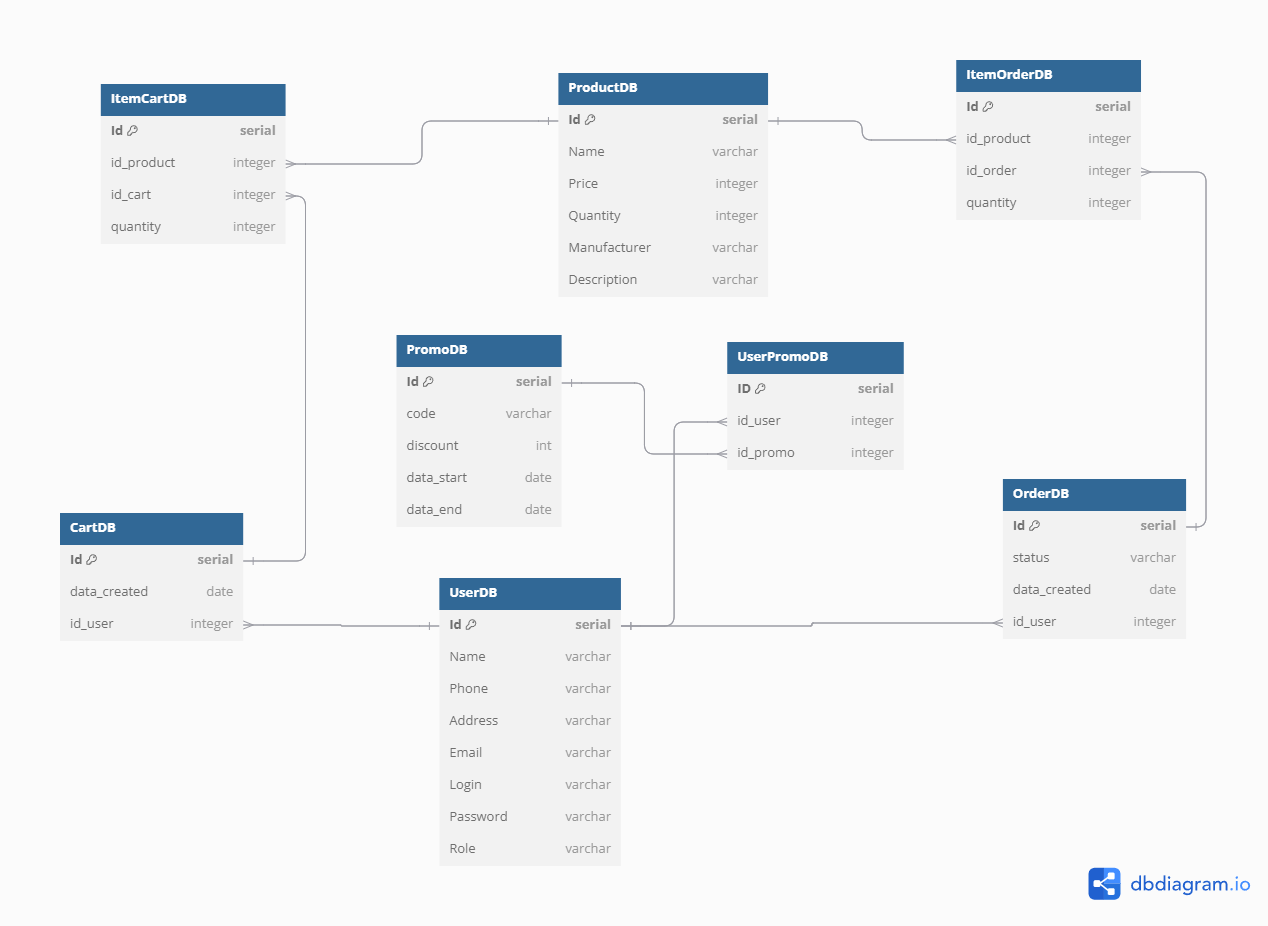
\includegraphics[width=1\linewidth]{img/er_db.png}
	\caption{Диаграмма базы данных}
	\label{img:er-db}
\end{figure}

На основе диаграммы сущностей-связей, приведенной на рисунке \ref{img:er-db}, определяются стуктуры столбцов, их типы.

\begin{table}[H]
	\begin{center}
		\caption{Сведение о таблице userdb}
		\begin{tabular}{|c|c|c|c|}
			\hline
			Столбец & Тип данных & Ограничения & Значение \\
			\hline
			id & serial & PK & Идентификатор \\
			\hline
			name & VARCHAR(50) & NOT NULL & имя \\
			\hline
			phone & VARCHAR(50) & NOT NULL & Номер телефона\\
			\hline
			address & VARCHAR(50) & NOT NULL & Адрес\\
			\hline
			email & VARCHAR(50) & NOT NULL & Почта \\
			\hline
			login & VARCHAR(50) & NOT NULL &  Логин \\
			\hline
			password & VARCHAR(50) & NOT NULL & Пароль \\
			\hline
			role & VARCHAR(50) & NOT NULL & Права доступа \\
			\hline			
		\end{tabular}
		\label{table:db:users}
	\end{center}
\end{table}

\begin{table}[H]
	\begin{center}
		\caption{Сведение о таблице promodb}
		\begin{tabular}{|c|c|c|c|}
			\hline
			Столбец & Тип данных & Ограничения & Значение \\
			\hline
			id & serial & PK & Идентификатор \\
			\hline
			code & VARCHAR(50) & NOT NULL & Код \\
			\hline
			discount & INT & NOT NULL & Акция\\
			\hline
			data\_start & DATE & NOT NULL & Дата начала\\
			\hline
			data\_end & DATE & NOT NULL &  Дата конца\\
			\hline			
		\end{tabular}
		\label{table:db:promodb}
	\end{center}
\end{table}

\begin{table}[H]
	\begin{center}
		\caption{Сведение о таблице productdb}
		\begin{tabular}{|c|c|c|c|}
			\hline
			Столбец & Тип данных & Ограничения & Значение \\
			\hline
			id & serial & PK & Идентификатор \\
			\hline
			name & VARCHAR(50) & NOT NULL & Название \\
			\hline
			price & INT & NOT NULL & Цена\\
			\hline
			quantity & VARCHAR(50) & NOT NULL & Количество на складе\\
			\hline
			manufacturer & VARCHAR(50) & NOT NULL &  Производитель\\
			\hline
			description & VARCHAR(50) & NOT NULL &  Описание\\
			\hline			
		\end{tabular}
		\label{table:db:productdb}
	\end{center}
\end{table}

\begin{table}[H]
	\begin{center}
		\caption{Сведение о таблице Cartdb}
		\begin{tabular}{|c|c|c|c|}
			\hline
			Столбец & Тип данных & Ограничения & Значение \\
			\hline
			id & serial & PK & Идентификатор \\
			\hline
			data\_created & DATE & NOT NULL & Дата создания \\
			\hline
			id\_user & INT & FK & Идентификатор пользователя\\
			\hline			
		\end{tabular}
		\label{table:db:Cartdb}
	\end{center}
\end{table}

\begin{table}[H]
	\begin{center}
		\caption{Сведение о таблице ItemCartdb}
		\begin{tabular}{|c|c|c|c|}
			\hline
			Столбец & Тип данных & Ограничения & Значение \\
			\hline
			id & serial & PK & Идентификатор \\
			\hline
			id\_product & VARCHAR(50) & FK & Идентификатор товары \\
			\hline
			id\_cart & INT & FK & Идентификатор корзины\\
			\hline
			Quantity & INT & NOT NULL & Количество\\
			\hline			
		\end{tabular}
		\label{table:db:ItemCartdb}
	\end{center}
\end{table}

\begin{table}[H]
	\begin{center}
		\caption{Сведение о таблице Orderdb}
		\begin{tabular}{|c|c|c|c|}
			\hline
			Столбец & Тип данных & Ограничения & Значение \\
			\hline
			id & serial & PK & Идентификатор \\
			\hline
			status & VARCHAR(50) & NOT NULL & Дата создания \\
			\hline
			data\_created & DATE & NOT NULL & Дата создания \\
			\hline
			id\_user & INT & FK & Идентификатор пользователя\\
			\hline
			id\_promo & INT & FK & Идентификатор промокода\\
			\hline			
		\end{tabular}
		\label{table:db:Orderdb}
	\end{center}
\end{table}

\begin{table}[H]
	\begin{center}
		\caption{Сведение о таблице ItemOrderdb}
		\begin{tabular}{|c|c|c|c|}
			\hline
			Столбец & Тип данных & Ограничения & Значение \\
			\hline
			id & serial & PK & Идентификатор \\
			\hline
			id\_product & INT & FK & Идентификатор товары \\
			\hline
			id\_order & INT & FK & Идентификатор заказа \\
			\hline
			quantity & INT & NOT NULL & Количество\\
			\hline		
		\end{tabular}
		\label{table:db:Orderdb}
	\end{center}
\end{table}

\subsection{Ролевая модель}
Создание ролей для каждой группы пользователей в базе данных
\begin{enumerate}
	\item Гость имеет право добавления в таблицу userdb;
	\item Клиент имеет право просмотра всех таблиц, добавления в таблицы cartdb, itemcartdb, orderdb, itemorderdb, удаления в таблицах cartdb, itemcartdb, изменения в таблице users;
	\item Поставщик имеет право просмотра, добавления, удаления всех таблиц, кроме таблицы userdb, cartdb, itemcartdb, promodb;
	\item Администратор имеет право просмора всех таблиц, добавления, изменения, удаления из всех таблиц.
\end{enumerate}
\newpage
\section{Триггеры}
Триггеры в PostgreSQL --- это инструмент для автоматизации определённых действий в базе данных, которые выполняются автоматически в ответ на события, такие как вставка, обновление или удаление данных \cite{4}. Основные особенности и преимущества использования триггеров в PostgreSQL:
\begin{enumerate}
	\item Триггеры позволяют автоматизировать задачи, такие как обновление связанных таблиц, ведение логов изменений или валидация данных, без необходимости вручную писать код в приложении для выполнения этих действий.
	\item  PostgreSQL триггеры могут срабатывать на различные операции (INSERT, UPDATE, DELETE), а также на уровне строк или таблиц. Это позволяет гибко настраивать, когда и как они должны выполняться.
	\item Триггеры могут быть настроены на выполнение как до выполнения операции (BEFORE), так и после неё (AFTER). Это даёт возможность, например, проверять или изменять данные до того, как они будут записаны в базу.
	\item Триггер проверяет каждую введенную команду, насколько она достоверна и реальна. Эта процедура помогает избежать ошибок в базе данных.
\end{enumerate}

В этом проекте используются триггеры, когда клиент размещает заказ, количество товара на складе автоматически уменьшается на количество товара в заказе.

Ниже, на рисунке \ref{img:trigger}, представлена схема вышеуказанного триггера.
\begin{figure}[ht!]
	\centering
	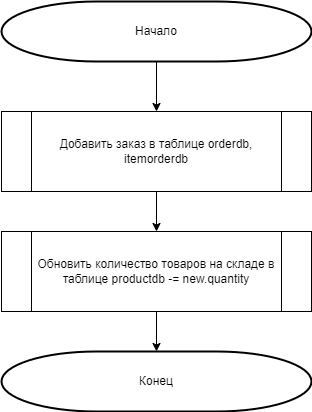
\includegraphics[width=0.65\linewidth]{img/trigger.png}
	\caption{Схема тригерра}
	\label{img:trigger}
\end{figure}

\clearpage
\section{Декомпозиция разрабатываемого \newline программного обеспечения}
На рисунке \ref{img:uml_class}, представлена схема UML-диаграмма классов приложения.
\begin{figure}[ht!]
	\centering
	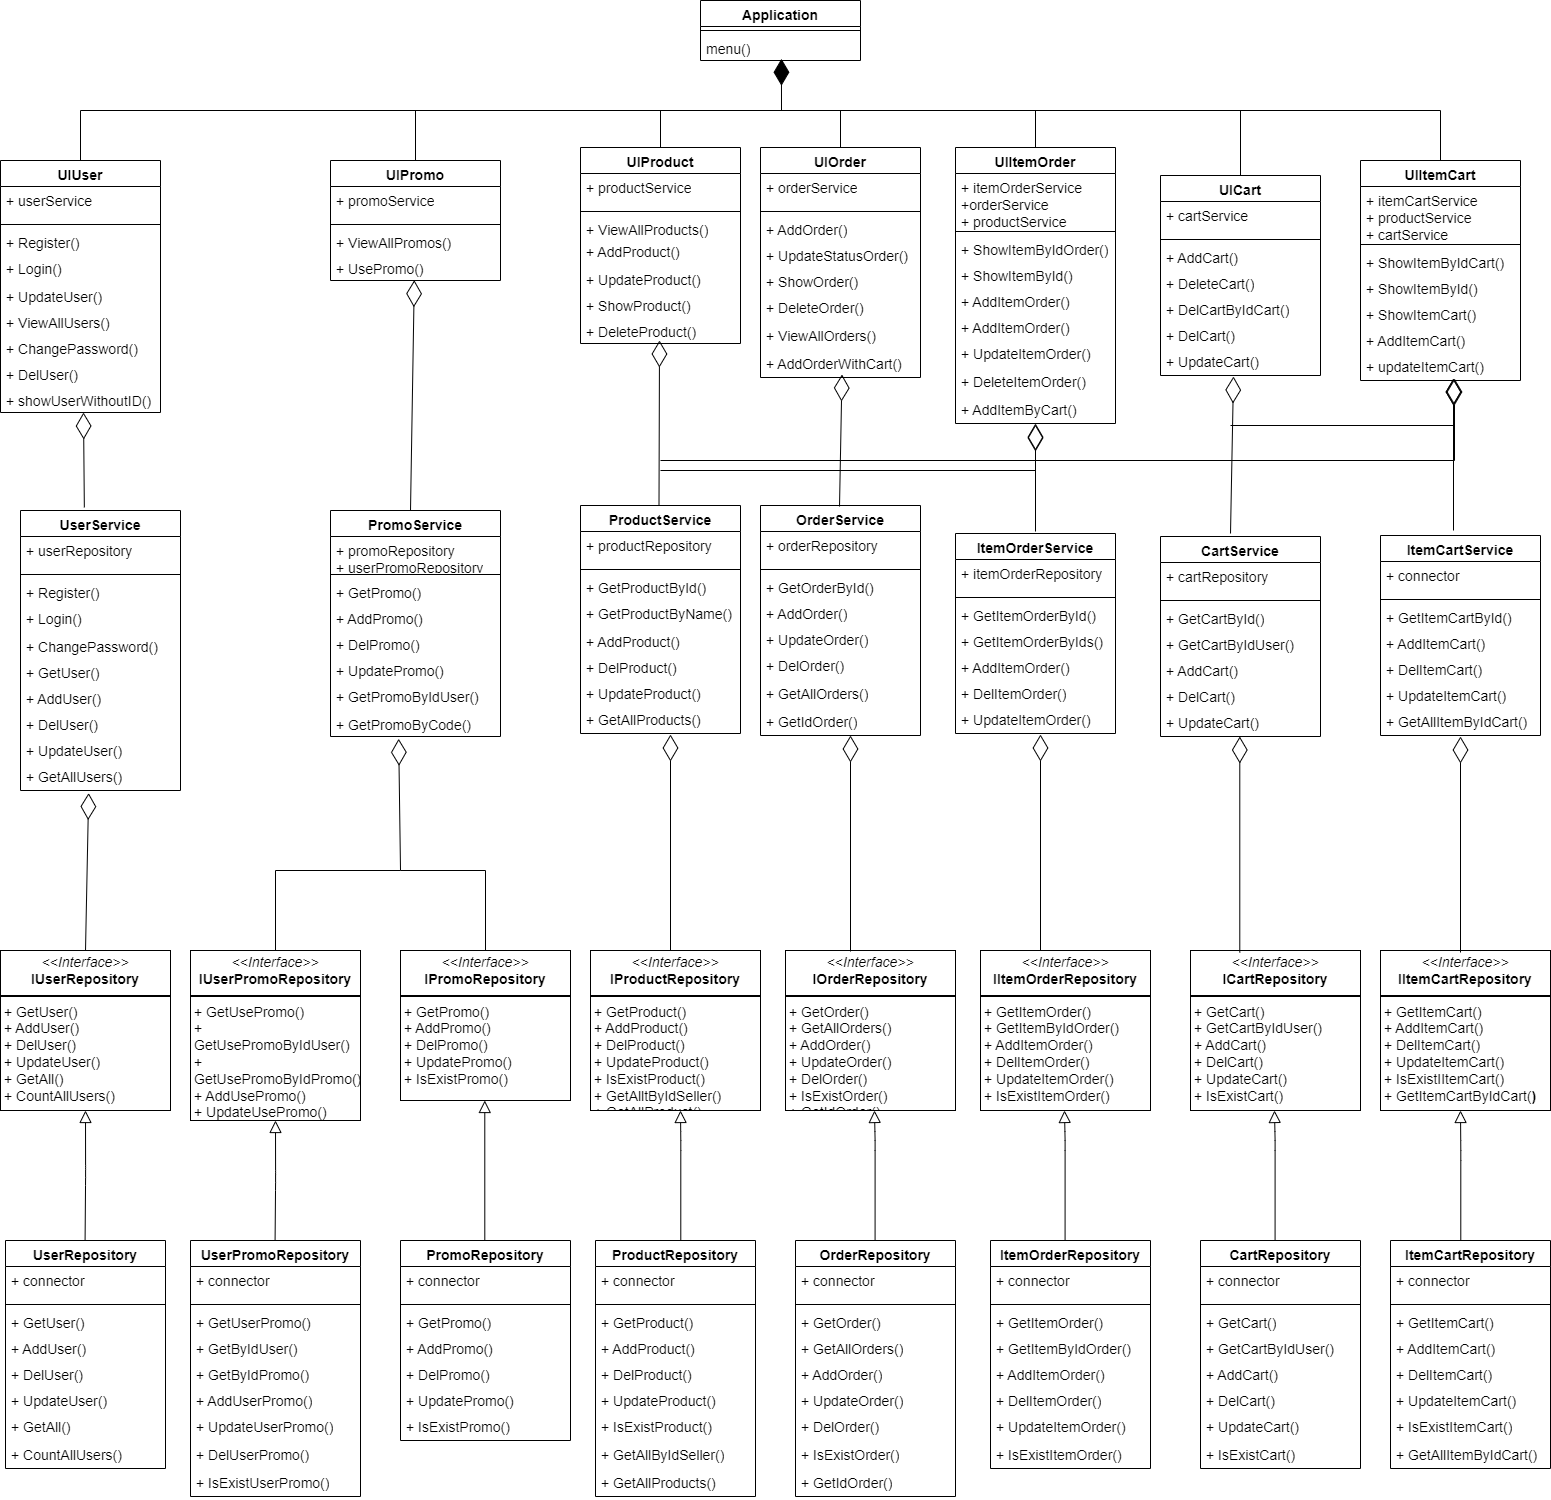
\includegraphics[height=1\linewidth]{img/UML_CLass.png}
	\caption{Диаграмма разработанного программного обеспечения}
	\label{img:uml_class}
\end{figure}

В программе реализованы следующие классы:
\begin{itemize}[label=---]
	\item class UserRepository, IUserRepository - это класс и интерфейс класса компонента для доступа к данным для сущности пользователей; 
	\item class PromoRepository, IPromoRepository - это класс и интерфейс класса компонента для доступа к данным для сущности промокодов; 
	\item class ProductRepository, IProductRepository -- это класс и интерфейс класса компонента для доступа к данным для сущности товаров;  
	\item class OrderRepository, IOrderRepository- это класс и интерфейс класса компонента для доступа к данным для сущности заказов; 
	\item class ItemOrderRepository, IItemOrderRepository - это класс и интерфейс класса компонента для доступа к данным для сущности деталей заказа; 
	\item class CartReposiotory, ICartReposiotory - это класс и интерфейс класса компонента для доступа к данным для сущности корзин; 
	\item class ItemCartRepository, IItemCartRepository - это класс и интерфейс класса компонента для доступа к данным для сущности деталей корзины;  
	\item class UserService, UserPromoService, PromoService, ProductService, \newline OrderService, ItemOrderService, CartService, ItemCartService: -- эти классы компонента бизнес-логики соответствующий сущностей: пользовотель, промокод, товар, заказ, деталь заказа, корзина, деталь корзины;
	\item class UIUser, UIUserPromo, UIPromo, UIProduct, UIOrder, UIItemOrder, UICart, UIItemCart -- эти классы графического пользовательского интерфейса соответствующий сущностей: пользовотель, промокод, товар, заказ, деталь заказа, корзина, деталь корзины.
\end{itemize}

\subsection*{Вывод} 
В этом разделе спроектирована база данных и приложение для доступа к ней. Был спроектирован триггер, осуществляющие автоматически пересчитывать количество товаров на складе при добавления заказов.
